\documentclass[conference]{IEEEtran}
% Build: latexmk -pdf main.tex   (tables and plot data come from generated/,
% produced by: python3 src/report/make_assets.py)
\usepackage[T1]{fontenc}
\usepackage{cite}
\usepackage{amsmath,amssymb}
\usepackage{booktabs}
\usepackage{multirow}
\usepackage{xcolor}
\usepackage{url}
\usepackage{tikz}
\usetikzlibrary{arrows.meta,positioning,fit,backgrounds}
\usepackage{pgfplots}
\pgfplotsset{compat=1.17}
\usepackage[hidelinks]{hyperref}

% \input is not expandable, so it breaks \bottomrule after it inside a tabular; the primitive works.
\makeatletter\newcommand{\inputtab}[1]{\@@input #1 }\makeatother
\newcommand{\lbl}[1]{\textsc{#1}}
\newcommand{\IO}{\lbl{io\_wait}}
\newcommand{\SCHED}{\lbl{sched\_wait}}
\newcommand{\CPU}{\lbl{syscall\_cpu}}
\newcommand{\IND}{\lbl{indeterminate}}

\begin{document}

\title{Fingerprinting I/O-Induced Application Stalls\\ by Fusing Syscall, Scheduler and Block-Layer eBPF Evidence}

\author{\IEEEauthorblockN{Tarun Sekar S.D \quad Karthick Krishna K \quad Rohit A \quad Raihan}
\IEEEauthorblockA{Operating Systems, Assignment 3}}

\maketitle

\begin{abstract}
When an application operation is slow, the cause may be storage, competition for the CPU, or the operation's own CPU and kernel work. Common tools look at one kernel layer at a time and cannot say which. We build an eBPF tool (libbpf CO-RE) that records syscall, scheduler and block-layer events for marked operations, splits each operation's wall time into on-CPU, runnable-wait, I/O-blocked and other-blocked time, and labels it \IO, \SCHED, \CPU, or \IND{} when no cause dominates. We grade the labels against the kernel's own per-thread accounting on 12 controlled workloads with injected disk delay (\texttt{dm-delay}). On 5,184 held-out operations, fused rules reach macro-F1 0.989 [0.979, 0.996], against 0.647 for the best syscall-only and 0.852 for the best block-only classifier. Allowing \IND{} cuts high-confidence errors from 18.0\% to 0.7\% at 17.4\% abstention. Fusion does not beat scheduler evidence alone while the kernel's \texttt{in\_iowait} flag is available; without it, fusion adds +0.109 macro-F1 for rules and +0.019 for a decision tree, both with confidence intervals above zero. Traced stall time matches the kernel within 125\,\textmu s at 0--20\,ms injected delay. The cost is a roughly fixed tens of microseconds of CPU per operation, negligible for millisecond stalls and dominant for microsecond operations.
\end{abstract}

\begin{IEEEkeywords}
eBPF, observability, I/O stalls, scheduling, performance diagnosis, Linux kernel
\end{IEEEkeywords}

%=====================================================================
\section{Problem Definition}
%=====================================================================
A slow read can mean three different things. The thread may be \emph{blocked on storage}; it may be \emph{runnable but waiting for a CPU} because other threads hold every core; or it may be \emph{running}, spending its time in user code or in the kernel's syscall path (copying from the page cache, for example). The fix is different in each case, so a diagnosis tool must say which one applies, and it must say so for the operation the developer cares about, not as a system-wide average.

Each kernel layer on its own gives a misleading answer. A long \texttt{read()} syscall looks the same whether the thread waited for the disk, waited for a CPU, or slept on a lock. Block-layer activity during the operation may belong to another process, or to write-back of data the application wrote long ago. Scheduler events show \emph{that} a thread was off the CPU, but not always \emph{why}. A tool that sees only one layer will therefore sometimes be confidently wrong.

We address the following problem: \emph{given an application operation with known start and end, attribute its wall time to I/O wait, scheduler wait or syscall/CPU work using kernel evidence collected with eBPF, decline to label it when the evidence does not support a single cause, and measure how often the result is correct against ground truth.}

%=====================================================================
\section{Objectives}
%=====================================================================
\begin{enumerate}
\item Build a reproducible eBPF tracer and collector that records syscall, scheduler, block and page-fault events for chosen processes, with per-type drop counters.
\item Build controlled workloads whose correct label and stall length are known, including negative controls where block activity is present but is not the cause.
\item Label each operation with rules and with a depth-limited decision tree, each with an abstaining (\IND) and a forced variant.
\item Test two hypotheses declared before the final runs:
  \textbf{H1}: fused evidence gives higher macro-F1 than any single source;
  \textbf{H2}: an abstention class lowers the rate of high-confidence errors.
\item Measure overhead (throughput, p99 latency, CPU per operation, collector CPU, dropped events) against a budget declared in advance: at most 10\% throughput loss and under 1\% dropped events.
\item Report ablations (no block, no scheduler, no \texttt{in\_iowait}, PID-only windows of 5/20/100\,ms) and the conditions under which the method fails.
\end{enumerate}

%=====================================================================
\section{Literature Survey}
%=====================================================================
\textbf{Joint user/kernel I/O tracing.} EZIOTracer~\cite{naas2021eziotracer} links user-level I/O calls to VFS, page-cache, file-system and block events per thread, matching them with a shared monotonic clock. We reuse that idea for our operation markers. EZIOTracer has no scheduler evidence, so it cannot separate storage wait from CPU starvation, and it does not classify: a person reads the trace. Its finding that buffered writes produce almost no synchronous block events is one of our negative controls.

\textbf{Syscall-level observability.} Rezvani et al.~\cite{rezvani2024ispass} show that eBPF syscall statistics can track request-level latency and throughput of latency-critical services without changing the application. They work with aggregate syscall statistics and do not attribute individual requests to a cause. DIO~\cite{esteves2023dio} intercepts 42 storage-related syscalls with eBPF, enriches them with kernel context such as file paths and offsets, and streams them to a search-and-dashboard backend, where a person diagnoses problems such as thread contention behind RocksDB tail latency. Its evidence is limited to the syscall layer, diagnosis is manual, and on RocksDB it costs a 1.37$\times$ slowdown and drops 3.5\% of events. Our syscall-only baseline represents this family.

\textbf{Off-CPU analysis.} wPerf~\cite{zhou2018wperf} records context switches, wakeups and interrupt handlers with kprobes (about 5\% overhead), models each I/O device as a pseudo-thread, and builds a wait-for graph to find the waiting events that bound a multi-threaded program's throughput. Its authors deliberately avoid syscall durations as a measure of I/O waiting because time inside a syscall may be data copying or contention; our syscall-only results confirm this. wPerf explains \emph{who waits for whom} across a whole program, whereas we label each operation and grade the label against ground truth. Off-CPU and block-latency tools in common use~\cite{gregg2019bpf} show each signal separately and leave the fusion to the user.

\textbf{Tracer fidelity and cost.} Machado et al.~\cite{machado2025snowflakes} compare five eBPF libraries under storage workloads and find that event loss and overhead differ widely; libbpf was the most efficient and among the most complete in events captured. We therefore use libbpf CO-RE~\cite{libbpf}, small fixed-size events and a ring buffer with in-kernel drop counters, and we report drops for every run.

\textbf{Gap.} Table~\ref{tab:related} summarises the comparison. No work we found fuses the three layers per operation, provides an explicit ``cannot tell'' outcome, and validates the labels and stall lengths against injected ground truth.

\begin{table}[t]
\centering
\caption{Prior work versus this work}
\label{tab:related}
\footnotesize
\setlength{\tabcolsep}{3pt}
\begin{tabular}{@{}lccccc@{}}
\toprule
 & Syscall & Sched & Block & Per-op label & Abstain / GT \\
\midrule
EZIOTracer~\cite{naas2021eziotracer} & \checkmark & -- & \checkmark & -- & -- / -- \\
Rezvani et al.~\cite{rezvani2024ispass} & \checkmark & -- & -- & -- & -- / \checkmark \\
DIO~\cite{esteves2023dio} & \checkmark & -- & -- & -- & -- / -- \\
wPerf~\cite{zhou2018wperf} & -- & \checkmark & IRQ & -- & -- / -- \\
Machado et al.~\cite{machado2025snowflakes} & \multicolumn{3}{c}{tracer cost only} & -- & -- / -- \\
\textbf{This work} & \checkmark & \checkmark & \checkmark & \checkmark & \checkmark{} / \checkmark \\
\bottomrule
\end{tabular}
\end{table}

%=====================================================================
\section{Methodology Used}
%=====================================================================
Fig.~\ref{fig:arch} shows the pipeline. All code, configuration and processed results are in the accompanying code archive.

\begin{figure}[t]
\centering
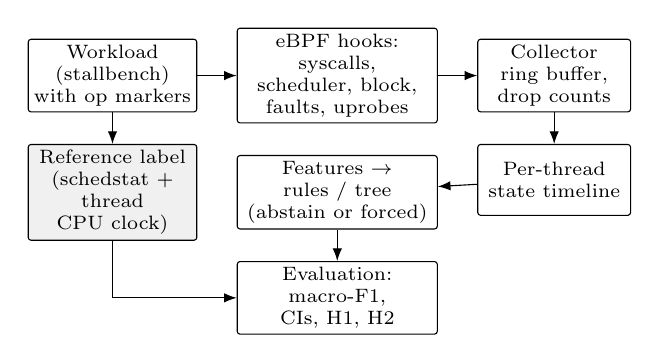
\begin{tikzpicture}[font=\scriptsize, node distance=4mm and 5mm,
  box/.style={draw, rounded corners=1pt, align=center, minimum height=9mm, inner sep=2pt},
  arr/.style={-{Latex[length=1.6mm]}}]
\node[box, text width=20mm] (wl) {Workload\\(stallbench)\\with op markers};
\node[box, right=of wl, text width=24mm] (k) {eBPF hooks: syscalls,\\scheduler, block,\\faults, uprobes};
\node[box, right=of k, text width=18mm] (c) {Collector\\ring buffer,\\drop counts};
\node[box, below=of wl, text width=20mm, fill=gray!12] (gt) {Reference label\\(schedstat +\\thread CPU clock)};
\node[box, below=of c, text width=18mm] (corr) {Per-thread\\state timeline};
\node[box, below=of k, text width=24mm] (cls) {Features $\rightarrow$\\rules / tree\\(abstain or forced)};
\node[box, below=of cls, text width=24mm, minimum height=6mm] (ev) {Evaluation: macro-F1,\\CIs, H1, H2};
\draw[arr] (wl) -- (k); \draw[arr] (k) -- (c); \draw[arr] (c) -- (corr);
\draw[arr] (corr) -- (cls); \draw[arr] (cls) -- (ev);
\draw[arr] (wl) -- (gt); \draw[arr] (gt) |- (ev);
\end{tikzpicture}
\caption{Pipeline. The workload marks each operation and records the kernel's own accounting as ground truth; the tracer's evidence is turned into a per-operation time split, features and a label.}
\label{fig:arch}
\end{figure}

\subsection{Workloads and ground truth}
A C program, \texttt{stallbench}, runs one of 12 workloads with 1, 4 or 16 threads and calls two non-inlined marker functions around each operation. I/O workloads: \texttt{direct\_read} (\texttt{O\_DIRECT}), \texttt{cold\_read} (page cache dropped), \texttt{sync\_write} (\texttt{write}+\texttt{fdatasync}), \texttt{mmap\_cold} (page faults on an unmapped file; our extension). Non-I/O workloads: \texttt{warm\_read}, \texttt{buffered\_write} and \texttt{mmap\_warm} (served from memory), \texttt{cpu} (10\,ms loop), \texttt{cpu\_contended} (same loop with hogs pinned to the same core), \texttt{sleep} (2\,ms \texttt{nanosleep}), \texttt{neighbor\_io} (CPU loop while another process reads the same disk), and \texttt{mixed} (a direct read followed by an equally long CPU loop, so that no cause dominates).

Every operation carries two labels. The \emph{design label} is what the workload was built to produce. The \emph{reference label}, our main ground truth, comes from the kernel's own per-thread accounting read around the operation: CPU time from \texttt{CLOCK\_THREAD\_CPUTIME\_ID} and run-queue delay from \texttt{/proc/thread-self/schedstat}~\cite{schedstats}; the rest of the wall time is blocked time. An operation is \IO{}, \SCHED{} or \CPU{} if that share exceeds 60\% of its wall time; blocked time counts as I/O only in workloads that issue I/O, so a dominant sleep is \IND. Reads are retried until consistent, since a preemption in the middle of a read can otherwise create milliseconds of false blocked time. In WSL the kernel's \texttt{sched\_clock} ran 0.92--1.04$\times$ the speed of \texttt{CLOCK\_MONOTONIC}; we measure this ratio at the start and end of every run, rescale, and flag runs where it drifts.

Delay is injected with \texttt{dm-delay}~\cite{dmdelay} on a loop-backed ext4 file system, so I/O waits are real and of known length despite the host's disk cache.

\subsection{Tracer and collector}
The eBPF program attaches to \texttt{raw\_syscalls} enter/exit, \texttt{sched\_switch} and \texttt{sched\_wakeup}, the block tracepoints \texttt{block\_bio\_queue}, \texttt{block\_rq\_issue} and \texttt{block\_rq\_complete}, user page faults, and uprobes on the two markers. Each event is a 48-byte record reserved and committed in a BPF ring buffer; failed reservations increment a per-CPU drop counter, reported per event type. On \texttt{sched\_switch} we record whether the outgoing task is preempted, its state, the kernel's \texttt{in\_iowait} flag and whether the incoming task is the idle task. Tasks are matched by namespace-local PIDs so that the tool works inside PID namespaces (WSL places user processes in one). Block requests are attributed to the submitting thread at queue time and also counted device-wide.

\subsection{Correlation}
For each thread we replay switch and wakeup events into a timeline with five states: \emph{run}, \emph{runqueue} (runnable, waiting for a CPU, including preemption), \emph{wake latency} (woken onto an idle CPU), \emph{blocked-I/O} (\texttt{in\_iowait} set) and \emph{blocked-other}. Wake latency is separate because under WSL, waking an idle CPU takes tens of microseconds (median 18--62\,\textmu s per wakeup across the blocking workloads at one thread), which the kernel counts as CPU time; treating it as contention mislabels uncontended I/O. Each operation's window, given by its markers, yields the shares of these states, syscall time and count, bytes submitted to the block layer by the thread, device-wide block completions, and page faults.

\subsection{Classifiers and baselines}
\emph{Fused rules} label an operation \SCHED{} if runqueue share exceeds 60\%; \IO{} if blocked-I/O share exceeds 60\% and the thread or device shows block activity (otherwise the evidence conflicts and the label is \IND); \CPU{} if run plus wake latency exceeds 60\%; and \IND{} otherwise, including when blocked time dominates but \texttt{in\_iowait} could not be read. The \emph{forced} variant always picks the largest share. A CART \emph{decision tree} (depth 4, minimum leaf 5) is trained per feature set with \IND{} as a class; it may also abstain when leaf purity falls below a threshold tuned on development runs. Its forced variant returns the most likely of the three causes in the leaf.

Each classifier is run on six feature sets: syscall only; block only (per-thread and device-wide variants); scheduler only; scheduler without \texttt{in\_iowait} (blocked time not split); fused; and fused without \texttt{in\_iowait}. The syscall rule reads a long syscall as I/O, the way a syscall-latency tool would.

\subsection{Evaluation protocol}
Runs, not operations, are split: repetitions 1--2 tune thresholds and train trees; repetitions 3--5 are test only. The configuration was frozen before the final runs. We report macro-F1 with 95\% bootstrap confidence intervals over test runs (1,000 resamples), accuracy, per-class precision and recall, abstention rate, and the \emph{high-confidence error rate}: the fraction of operations given a wrong non-\IND{} label. H1 and H2 use paired bootstrap differences. A transfer test trains I/O workloads on 64\,KiB sequential I/O and tests on 16\,KiB random I/O.

%=====================================================================
\section{Experimental Results}
%=====================================================================
\subsection{Setup}
Experiments ran on WSL2 (kernel 6.6.87, Ubuntu 24.04) on an 8-thread Intel i7-1065G7 with 7.7\,GiB RAM, with 2\,ms injected delay. The final matrix has 204 runs (12 workloads $\times$ 3 thread counts $\times$ 5 repetitions, plus 24 transfer runs), all completed, and 9,792 operations: 4,027 \IO, 819 \SCHED, 3,440 \CPU{} and 1,506 \IND{} by the reference label. The tracer produced 766,242 events and dropped 0.54\%.

\subsection{Accuracy and H1}
Table~\ref{tab:main} and Fig.~\ref{fig:f1} give the results on the 5,184 test operations. Fused classifiers reach macro-F1 0.989 (rules) and 0.986 (tree). Syscall-only evidence is the weakest: the naive rule scores 0.444 and even a trained tree only 0.647, because a long syscall looks the same for disk, sleep and CPU queueing. Block-only evidence scores at most 0.852: it labels \texttt{mixed} operations as \IO{} because it sees the read but not the CPU half (39\% of its errors), and it cannot separate CPU work from scheduler wait in \texttt{cpu} and \texttt{cpu\_contended} (37\%); \texttt{neighbor\_io} accounts for 13\%.

H1 holds against syscall-only and block-only evidence (Table~\ref{tab:h1}). It does \emph{not} hold against scheduler-only evidence: with \texttt{in\_iowait}, the difference is exactly zero, and the trained fused tree splits on scheduler time shares and the operation's wall time, with one split on syscall share and none on block features. The flag already tells the scheduler \emph{why} a thread blocked. Removing it shows what the other layers contribute: scheduler-only rules fall to 0.879, and fusion then adds +0.109 [+0.051, +0.176] for rules and +0.019 [+0.005, +0.038] for the tree, because the thread's own block requests separate a disk wait from a sleep. The same holds against the design label (+0.097 and +0.021). We conclude that fusion matters when the scheduler cannot see the cause of a block.

\begin{table*}[t]
\centering
\caption{Test-set results (5,184 operations, 108 runs) against the reference label. Hc-err: high-confidence error rate, with abstention and forced. Last column: macro-F1 against the design label.}
\label{tab:main}
\footnotesize
\begin{tabular}{@{}llccccccc@{}}
\toprule
Evidence & Model & Macro-F1 & 95\% CI & Acc.\,(\%) & Abstain\,(\%) & Hc-err\,(\%) & Hc-err forced\,(\%) & Design F1 \\
\midrule
\inputtab{generated/tab_main.tex}
\bottomrule
\end{tabular}
\end{table*}

\begin{figure}[t]
\centering
\begin{tikzpicture}
\begin{axis}[
  width=\columnwidth, height=4.3cm, ybar, bar width=6pt,
  ymin=0, ymax=1.05, ylabel={Macro-F1}, ylabel style={font=\scriptsize},
  xtick=data, xticklabels={Syscall, Block, Sched, {Sched\\no iowait}, {Fused\\no iowait}, Fused},
  xticklabel style={font=\scriptsize, align=center}, yticklabel style={font=\scriptsize},
  legend style={font=\scriptsize, at={(0.5,1.03)}, anchor=south, legend columns=2, draw=none},
  ymajorgrids, grid style={gray!25}, enlarge x limits=0.1]
\addplot+[fill=gray!40, draw=black, error bars/.cd, y dir=both, y explicit, error bar style={black}]
  table[x=idx, y=rules, y error plus=rules_hi, y error minus=rules_lo]{generated/f1bars.dat};
\addplot+[fill=black!75, draw=black, error bars/.cd, y dir=both, y explicit, error bar style={black}]
  table[x=idx, y=tree, y error plus=tree_hi, y error minus=tree_lo]{generated/f1bars.dat};
\legend{Rules, Tree}
\end{axis}
\end{tikzpicture}
\caption{Macro-F1 by evidence source, with 95\% bootstrap CIs (test runs, reference label).}
\label{fig:f1}
\end{figure}

\begin{table}[t]
\centering
\caption{H1: fused minus single-source macro-F1 with 95\% CI (reference label). $^*$Both without \texttt{in\_iowait}.}
\label{tab:h1}
\scriptsize
\setlength{\tabcolsep}{2.5pt}
\begin{tabular}{@{}lcccc@{}}
\toprule
 & \multicolumn{2}{c}{Rules} & \multicolumn{2}{c}{Tree} \\
\midrule
\inputtab{generated/tab_h1.tex}
\bottomrule
\end{tabular}
\end{table}

\subsection{Abstention (H2)}
H2 is supported (Table~\ref{tab:h2}). Forced to choose, the fused classifiers are confidently wrong on 18.0--18.4\% of operations, almost all of them the 17.7\% of test operations with no dominant cause (\texttt{mixed}, \texttt{sleep}), which a forced classifier cannot label correctly. With \IND{} available they abstain on 17--18\% and their high-confidence error falls below 1.3\%; every confidence interval of the difference excludes zero. The fused tree's confusion matrix (Table~\ref{tab:conf}) shows that the remaining errors are between neighbouring classes near the 60\% boundary: \CPU{} operations with some run-queue time, and \IND{} operations whose CPU share is just above the threshold. No operation is wrongly labelled \IO.

\begin{table}[t]
\centering
\caption{H2: high-confidence error (\%) forced vs.\ abstaining}
\label{tab:h2}
\scriptsize
\setlength{\tabcolsep}{3pt}
\begin{tabular}{@{}lcccc@{}}
\toprule
Model & Forced & Abstaining & Abstain & Diff.\ 95\% CI \\
\midrule
\inputtab{generated/tab_h2.tex}
\bottomrule
\end{tabular}
\end{table}

\begin{table}[t]
\centering
\caption{Confusion matrix, fused tree (rows: reference label)}
\label{tab:conf}
\scriptsize
\begin{tabular}{@{}lcccccc@{}}
\toprule
 & I/O & Sched & CPU & Indet. & Prec. & Recall \\
\midrule
\inputtab{generated/tab_confusion.tex}
\bottomrule
\end{tabular}
\end{table}

\subsection{Tracer fidelity and stall duration}
Over the same window, the tracer's time split agrees with the kernel's accounting to a median absolute error of 0.02--1.1 percentage points per workload. Fig.~\ref{fig:delay} varies the injected delay. Traced I/O-blocked time per operation tracks the kernel's blocked time within 2--125\,\textmu s at every level. Note that \texttt{dm-delay} quantises delays in this environment: a nominal 5\,ms becomes about 11\,ms and 20\,ms about 23\,ms. Measured in units of the effective delay, a direct or cold read waits 1.05--1.11 times, a synchronous write 2.2--2.4 times (data then journal), a cold \texttt{mmap} access 17 times (one fault per read-ahead window), and a sleep zero times.

\begin{figure}[t]
\centering
\begin{tikzpicture}
\begin{semilogyaxis}[
  width=\columnwidth, height=4.4cm, xlabel={Nominal injected delay (ms)}, ylabel={I/O-blocked per op (ms)},
  xtick={0,5,20}, label style={font=\scriptsize}, tick label style={font=\scriptsize},
  legend style={font=\scriptsize, at={(0.5,1.03)}, anchor=south, legend columns=4, draw=none},
  ymajorgrids, grid style={gray!25}]
\addplot+[mark=o, black] table[x=delay, y=trace]{generated/delay_mmap_cold_t1.dat};
\addplot+[mark=square, black, dashed] table[x=delay, y=trace]{generated/delay_sync_write_t1.dat};
\addplot+[mark=triangle, black, dotted] table[x=delay, y=trace]{generated/delay_direct_read_t1.dat};
\addplot+[only marks, mark=x, red, mark size=3pt] table[x=delay, y=kernel]{generated/delay_mmap_cold_t1.dat};
\addplot+[only marks, mark=x, red, mark size=3pt, forget plot] table[x=delay, y=kernel]{generated/delay_sync_write_t1.dat};
\addplot+[only marks, mark=x, red, mark size=3pt, forget plot] table[x=delay, y=kernel]{generated/delay_direct_read_t1.dat};
\legend{mmap\_cold, sync\_write, direct\_read, kernel}
\end{semilogyaxis}
\end{tikzpicture}
\caption{Traced I/O-blocked time per operation (lines) and the kernel's blocked time (crosses) against injected delay, one thread. \texttt{sleep} stays at 0 and is not shown on the log scale.}
\label{fig:delay}
\end{figure}

\subsection{Ablations and sensitivity}
Table~\ref{tab:abl} lists the ablations for the fused tree. Removing block or syscall events changes nothing, while removing scheduler events costs 0.10 macro-F1; the scheduler layer carries the signal whenever \texttt{in\_iowait} is present. Without markers, the tool must cut each thread's timeline into fixed windows (PID-only mode) and macro-F1 falls to 0.809 at 5\,ms and about 0.89 at 20--100\,ms windows: short windows split operations, long windows mix them. The results do not depend on runs with dropped events or clock drift (0.984 on the 95 test runs with neither, 88\% of test operations), on operations near the 60\% boundary, or on I/O size and pattern (97.6\% transfer accuracy without \texttt{in\_iowait}; with it, transfer is perfect).

\begin{table}[t]
\centering
\caption{Ablations and sensitivity, fused tree (test runs)}
\label{tab:abl}
\scriptsize
\setlength{\tabcolsep}{3pt}
\begin{tabular}{@{}lcc@{}}
\toprule
Variant & Macro-F1 & 95\% CI \\
\midrule
\inputtab{generated/tab_ablation.tex}
\bottomrule
\end{tabular}
\end{table}

\subsection{Overhead}
Table~\ref{tab:ovh} compares tracing on and off, five interleaved repetitions each, with collector output in binary and no ground-truth reads. The tool adds a roughly fixed 21--45\,\textmu s of CPU per memory-served operation and 58--195\,\textmu s per disk operation, which also pays for scheduler and block events; most of it is the two marker uprobes, which cost about 7--10\,\textmu s each under WSL. Operations lasting milliseconds stay within the 10\% budget (\texttt{sleep} +4\%, \texttt{sync\_write} about 1\%); the 10\,ms CPU loop loses 1.5\% at 4 threads and a noisy 18.7\% (range $-25$ to $+56$\%) at one thread. Operations of a few microseconds lose 61--92\% throughput, and disk reads lose 13--27\%; a second untraced \texttt{direct\_read} run already differed from the first by 41\%, so the disk-read figure is uncertain. With the default 256\,KiB buffer, drops exceed 1\% only for the microsecond workloads (\texttt{warm\_read} at 1 and 4 threads, \texttt{buffered\_write} at 4); a 4\,MiB buffer removes them for \texttt{warm\_read} at 4 threads, the case we tested. Removing the markers cuts the added CPU per \texttt{warm\_read} from 21 to 7\,\textmu s.

\begin{table}[t]
\centering
\caption{Overhead, tracing on vs.\ off (median of 5 runs). Bold: over the 10\% budget. CPU: added CPU per op (\textmu s); Coll.: collector CPU (\% of one core)}
\label{tab:ovh}
\scriptsize
\setlength{\tabcolsep}{2.5pt}
\begin{tabular}{@{}lcccccc@{}}
\toprule
Workload & Thr & Tput loss\,\% & p99 +\% & CPU & Coll.\,\% & Drops\,\% \\
\midrule
\inputtab{generated/tab_overhead.tex}
\bottomrule
\end{tabular}
\end{table}

\subsection{Second environment}
We repeated the final matrix, the delay sweep and the overhead runs unchanged in an Ubuntu 24.04 VM (stock kernel 6.8, 4 vCPUs, 4\,GiB) under QEMU/KVM, with \texttt{dm-delay} on a separate virtual disk whose host cache is off. All 204 matrix runs completed with no dropped events and 2 drift-flagged runs (WSL: 0.54\% and 26). Table~\ref{tab:robust} shows that the conclusions hold: fused rules reach 0.971 [0.958, 0.980], fusion beats syscall-only and block-only evidence, it adds +0.111 [+0.056, +0.171] over scheduler evidence without \texttt{in\_iowait}, and abstention cuts high-confidence errors from 19.2\% to 1.4\%. Rules tuned on WSL runs score the same in the VM, but the tree trained on WSL without \texttt{in\_iowait} falls to 0.695: its learned timing thresholds do not carry over, while rules on time shares do. Traced I/O-blocked time matches the kernel within 422\,\textmu s; here 5\,ms of injected delay adds about 5.7\,ms per read, against about 11\,ms under WSL, so that excess is specific to the WSL environment; we did not establish its cause. Overhead is higher: the two marker uprobes add about 100\,\textmu s per operation under nested virtualisation, so even \texttt{sleep} and \texttt{sync\_write} lose 10--30\% throughput, and run-to-run noise is large.

\begin{table}[t]
\centering
\caption{Macro-F1 on test runs in WSL (kernel 6.6) and the VM (kernel 6.8); last column: classifiers trained on WSL runs, tested in the VM}
\label{tab:robust}
\scriptsize
\setlength{\tabcolsep}{3pt}
\begin{tabular}{@{}lccc@{}}
\toprule
Classifier & WSL & VM & VM, WSL-trained \\
\midrule
\inputtab{generated/tab_robust.tex}
\bottomrule
\end{tabular}
\end{table}

\subsection{Ethical and privacy safeguards}
The tracer records only timestamps, process and thread IDs, CPU, syscall numbers and return values, scheduler state, device numbers, sectors, byte counts and page-aligned fault addresses. It never reads file contents, file names, syscall arguments or buffers; for tasks outside the workload it keeps at most a numeric ID, never a name or command line. Cache dropping and delay injection ran only in disposable environments (WSL and a VM), on a loop file and a virtual test disk, never on a production system.

\subsection{Threats to validity}
The reference label comes from scheduler accounting, so scheduler features agree with it partly by construction; we therefore also report the design label, which agrees with the reference on 94.9\% of operations (93.3\% in the VM) and gives the same conclusions. All workloads are synthetic and single-purpose. Both environments are virtualised; bare-metal hardware and other file systems remain untested.

%=====================================================================
\section{Conclusion}
%=====================================================================
We built and evaluated an eBPF tool that labels individual operations as I/O-wait, scheduler-wait or syscall/CPU dominated, or declines to decide. Against the kernel's own accounting it reaches macro-F1 0.989, far above syscall-only (0.647) and block-only (0.852) evidence, and abstention lowers high-confidence errors from 18\% to under 1\%. Fusion pays off when the scheduler does not know why a thread blocked; while the kernel's \texttt{in\_iowait} flag is available, scheduler evidence alone is as good. Precise operation boundaries are worth about 0.1 macro-F1 over fixed windows, but their probes cost tens of microseconds per operation, so the tool suits diagnosing millisecond-scale stalls rather than always-on tracing of microsecond operations. Future work: lighter markers (USDT or kernel-side boundaries), real applications, and asynchronous I/O (\texttt{io\_uring}), where the thread that waits is not the one that submitted the request. The main conclusions held in a second environment (a kernel 6.8 VM).

\bibliographystyle{IEEEtran}
\bibliography{refs}

\end{document}
